\section{Automatic Control of IRIS Drone}
The team members responsible for this part of the project is Mikkel Jaedicke and Jens-Jakob Bentsen.
\subsection{Introduction}
As stated in the problem formulation the UAV needs to be controlled automatically from an external computer. This chapter seeks to show how this can be done. It will also tell about the IRIS UAV in general, different software solutions and steps needed to be done in order to have a successful flight. To fulfill the project formulation there is also a need for a program that uses the found coordinates of the drone to calculate control signals to the UAV. This chapter will explain how such a program could be developed. 

The chapter also describes two weather aviation protocols, METAR and TAF, and how they can be used in this project.

\subsection{General IRIS prerequisites}
\subsubsection{Firmware and Offboard Control Software}
The IRIS drone is equipped with a Pixhawk PX4 autopilot module, which is a \SI{68}{\mega\hertz} Cortex M4F CPU along with 3D accelerometer, gyroscope, magnetometer and barometer. It is built by Pixhawk and is a open-source hardware and software project.

The PX4 runs a open-source Real Time Operation System (RTOS) called NuttX. On top of NuttX runs a PX4 middleware layer providing drivers and a micro object request broker (uORB) for communication between tasks.

On top of the middleware layer runs a collection of tasks called the flight stack. It includes all the applications that is needed for the UAV to fly. There are two different flight stacks available for the PX4: The Pixhawk flight stack and the APM flight stack. They are developed by two different communities, but both flight stacks run on top of the PX4 middleware on NuttX. The IRIS UAV is, by default, shipped with the APM flight stack, but PX4 flight stack also has special settings for the IRIS UAS. 

The PX4 dev team has developed an offboard control software station called QGroundControl. QGroundControl runs on Windows, Linux and OS X. Features includes calibration of the UAV and RC controller, flashing firmware, real-time plotting of sensor and telemetry data, logging of sensor log and waypoint navigation. 

The APM dev team's newest offboard control software station is APM Planner 2.0, which also runs on Windows, Linux and OS X. It has a lot of the same features as QGroundControl including the most important ones: calibration of the UAV and RC controller, flashing firmware and waypoint navigation.

\subsubsection{Different Flight Modes}
There are a number of different flight modes for both Pixhawk flight stack and APM flight stack. They are similar, but not identical. Some of the important APM flight modes will be explained here. 

\emph{\textbf{Acro mode}}\\
Acro mode is a difficult mode to fly the UAV in. The throttle is completely manual with no compensation. The RC sticks control the angular velocity of the UAV; when the sticks are released the UAV will maintain its attitude, which makes it hard to fly. Acro mode is not recommended to beginners as they are almost guaranteed a crash.

\emph{\textbf{Stabilize mode}}\\
Stabilize mode is more beginner friendly, because the autopilot on the UAV will do more controlling than in acro mode. The UAV is flown manually, but when the pitch and roll sticks are released the autopilot will try to level the roll and pitch axis automatically. The throttle stick controls the motor speed directly, which means that a constant adjustment of the throttle stick is needed to fly.

\emph{\textbf{AltHold mode}}\\
Altitude-hold mode is identical to stabilize mode in roll, pitch and yaw. The difference is the throttle stick. Altitude-hold mode will try to maintain a constant altitude, while the throttle stick is released. When the throttle stick is in the upper position the UAV will climb and when the stick is in the down position the UAV will descent. 

It is important to note that the autopilot uses a barometer to determine its altitude. This means that if air pressure is changing due to extreme weather or other events AltHold mode will not be a good flight mode. The PID constants for this mode may also need to be tuned, which can be done in APM Planner.

\emph{\textbf{Auto mode}}\\
Auto mode is a mode, where the UAV will follow a preprogrammed path of waypoints. It is possible to switch to this mode on the ground or in the air. It is always possible for the pilot to retake control of the UAV by switching to e.g. stabilize mode. The path of waypoints can be uploaded to the UAV by using APM Planner.

\emph{\textbf{Land mode}}\\
Land mode is a flight mode that attempts to bring the UAV to land. Throttle is controlled by the autopilot, while yaw, pitch and roll are controlled as in stabilize mode. In land mode the UAV will automatically disarm when it lands.

\subsubsection{Initial Setup for Flight}
Before flight the UAV and the RC controller needs to be calibrated. This can be done with both QGroundControl and APM Planner, depending on the firmware on the UAV.
Both QGroundControl and APM Planner will guide the user through the calibration. The RC controller also needs to be calibrated before flying with the UAV. The user is also guided through this process. Both calibrations are straightforward processes.

\subsubsection{Flights}
Test flights were made with both Pixhawk flight stack and APM flight stack. We had major problems with the setup of both systems. When the setups were set up properly we had good test flights with both flight stacks. No big differences were noticed during the test flights.

\subsection{Automatic Route flight/planning}
\subsubsection{Weather forecast - TAF and METAR}
The application states that the UAV should be able to take off on its own at a predetermined time. However, weather may not always be in flight condition. To take this into account the control-computer should be able to analyze the weather.

To accomplish this, the computer should be able to extract the latest weather forecasts.

\emph{\textbf{TAF - Terminal Aerodome Forecast}}\\
TAF is a compact message form stating the weather forecast every 6 hours. It applies to a 24--30 hour window and within a radius of roughly \SI{8}{\kilo\meter} from the airport of which the forecast have been made. 
TAF weather forecasts rely on human resources and therefore they are not updated as much as its counterpart the METAR. 

Example:\\
\verb|TAF|\\
\verb|KXYZ 051730Z 0518/0624 31008KT 3SM -SHRA BKN020|\\
\verb|     FM052300 30006KT 5SM -SHRA OVC030|\\
\verb|     PROB30 0604/0606 VRB20G35KT 1SM TSRA BKN015CB|\\
\verb|     FM060600 25010KT 4SM -SHRA OVC050|\\
\verb|     TEMPO 0608/0611 2SM -SHRA OVC030|\\
\verb|     RMK NXT FCST BY 00Z=|\\

Decoding of TAF:

\begin{tabular}{ll}
	\toprule
	\textbf{Value} & \textbf{Meaning}                    \\\midrule
	TAF            & Message format                      \\
	KXYZ           & Airport indicator                   \\
	051730Z        & Day and Time of message ie. "5th day of month at 1730" Zulu time \\
	
	0518/0624      & Indicates timeslot for forecast ie. From the 5th at 18:00 to the 6th at 24:00 \\
	31008KT        & Wind is from 310 degrees at 8 knots \\
	3SM            & Visibility is 3 miles               \\
	-SHRA          & Light intensity Showering Rain      \\
	BKN020         & Broken ceiling at 2000 feet         \\\bottomrule
\end{tabular}
~\\
\emph{\textbf{ METAR - METeorological Aerodrome Report}}

METAR is a more dense version of TAF and is issued once an hour; however if visibility is below \SI{5}{\kilo\meter} or clouds get under 1000 ft METAR will be issued every half an hour. The message is published at hh:50 so at 00:50, 01:50, \ldots , 23:50. METAR is only representative for the weather 2 hours ahead.

Format:
METAR [ID] [time group] [wind] [visibility] [clouds] [temperature and dewpoint] [air pressure]

Example:\\
\verb|2015/05/10 08:20|\\
\verb|EKOD 100820Z 29015KT 9999 FEW016 BKN022 BKN027 10/08 Q1018|

\begin{tabular}{ll}
	\toprule
	\textbf{Value} & \textbf{Meaning}                            \\\midrule
	EKOD           & Odense Airport ID                           \\
	100820Z        & Time Indicator: 10th at 08:20 zulu          \\
	29015KT        & Winddirection 290 at 15 Knots               \\
	9999           & Visibility > 10000 meters                   \\
	FEW016         & Few cloud at 1600 feet                      \\
	BKN022         & Broken Clouds at 2200 ft                    \\
	BKN027         & Broken Clouds at 2700 ft                    \\
	10/08          & 10 degrees temperature / 8 degrees dewpoint \\
	Q1018          & Air Pressure is 1018 hPa                    \\\bottomrule
\end{tabular}
~\\~\\
METAR may also contain extra information like forecast of rain, snow, thunder etc. The codes can be seen in figure \vref{fig:metar_table}.

\begin{figure}
	\centering
	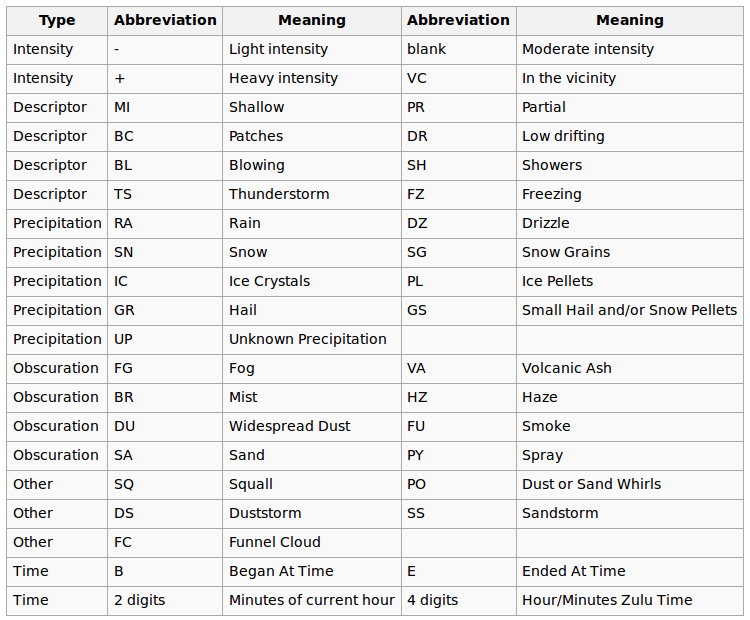
\includegraphics[width=0.8\textwidth]{imgs/metar_table}
	\caption{METAR translate table}
	\label{fig:metar_table}
\end{figure}

The message can additionally have one or more of the four following types:
\begin{enumerate}
	\item \textbf{CAVOK:} Perfect Weather or No weather (\textbf{C}eiling \textbf{A}nd \textbf{V}isibility \textbf{OK})
	\item \textbf{BECMG:} Means that the weather will be as stated shortly (\textbf{Bec}o\textbf{m}in\textbf{g})
	\item \textbf{TEMPO:} When weather is at its extreme (\textbf{Tempo}rary)
	\item \textbf{NOSIG:} \textbf{No sig}nificant changes the next 2 hours
\end{enumerate}

TAFs and METARs can be found in various locations online like:
\begin{itemize}
	\item \url{https://www.flygmet.dk/Flygmet/pages/login.jsp}
	\item \url{http://weather.noaa.gov/pub/data/observations/metar/stations/}
	\item \url{http://www.dmi.dk/vejr/i-luften/metar-og-taf/}
\end{itemize}

METAR for Odense airport:
\url{http://weather.noaa.gov/pub/data/observations/metar/stations/EKOD.TXT}

To sum up, METAR contains all the information we need. The information of greatest interest is the wind speed as we would like to be able to land securely on the platform. Also rain is greatly depreciated.\\
\emph{\textbf{Program for decoding METAR}}

A Python script for decoding METAR can be found at \url{http://sourceforge.net/projects/python-metar/}. The script downloads METAR from the \url{http://weather.noaa.gov/pub/data/observations/metar/stations/} website and converts it to an easy readable forecast. The webpages has a simple \verb|.TXT| file for each airport containing the latest METAR. The airports are indexed by their ICAO (International Civil Aviation Organization) airport code in caps. Hence Odense Airport becomes "EKOD" and the URL becomes \url{http://weather.noaa.gov/pub/data/observations/metar/stations/EKOD.TXT}.

\begin{figure}
	\centering
	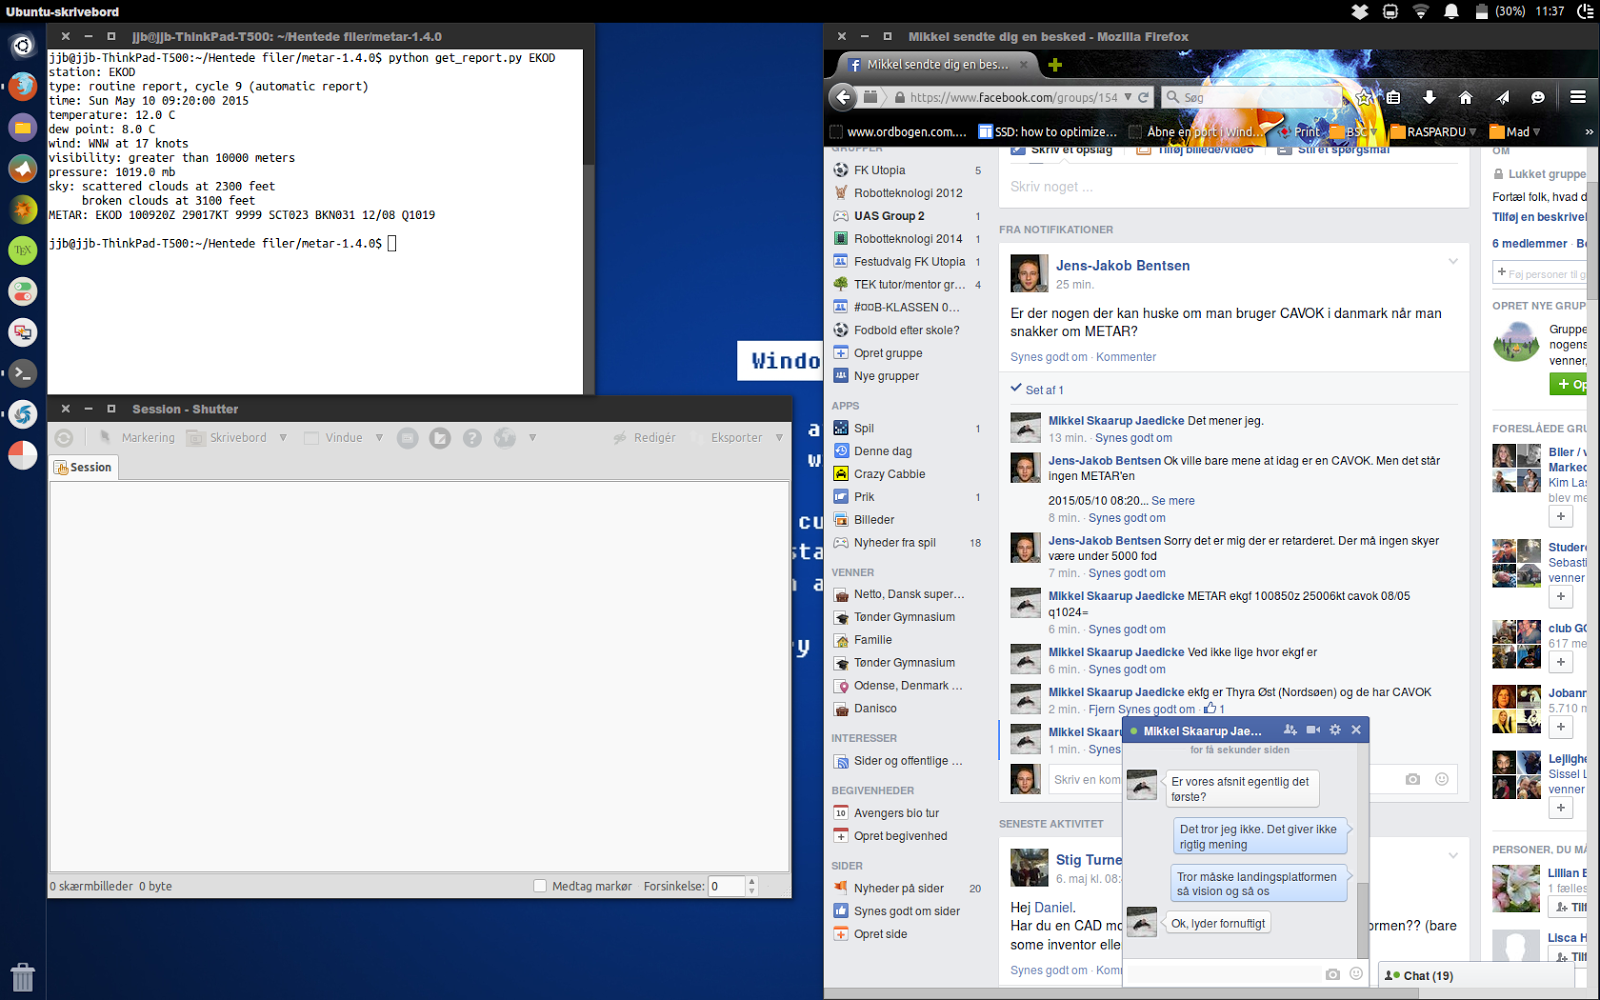
\includegraphics[width=0.8\textwidth, clip=true, trim=1.5cm 21.3cm 35.7cm 0.8cm]{imgs/metar_download}
	\caption{Output from the Python script \texttt{get\_report.py} called with the argument for Odense Airport "EKOD"}
\end{figure}
It is desired to used a modified version of this script to tell whether or not to lift off and whether or not to abort mission and return to station.
\subsection{Automatic Landing}
\subsubsection{MAVROS and the MavLink Protocol}
The micro air vechicle link, MAVLink, is a protocol used for communication between unmanned vehicles and ground control stations and in the intercommunication system within the vehicle itself. The latest message set can be found at \url{https://pixhawk.ethz.ch/mavlink/}. The MAVLink is often used to stream data containing state and whereabouts of the unmanned vehicle and is used by a ground control to enable auto piloting. 

%In the figure below we see a possible setup between the software Qgroundcontrol and an unmanned system %Figure gone missing? --mhs

MAVRos is a library implementing the MAVLink in ROS. MAVRos has been implemented to support mainly the native PIXHAWK firmware and the Arducopter firmware for APMplanner.
The MAVRos for Arducopter has implemented the possibility for a so called RC-override which has been banned from the native PIXHAWK firmware. The RC-override does not surprisingly overwrite the signals coming from the manual radio control unit.

\subsubsection{MAVROS usage}
To facilitate MAVROS the following should be installed.
\begin{itemize}
	\item Ubuntu 14.04 LTS
	\item ROS
	\item MAVLink/MAVRos
\end{itemize}

The first two can easily be found and installed. MAVLink was installed using this command in a terminal in Ubuntu:\\
\verb|$ sudo apt-get install ros-indigo-mavros ros-indigo-mavros-extras|

To see that everything is working the following steps should be applied:
\begin{enumerate}
\item Make sure that the drone is turned on and that the radio links has been paired. Open a supported groundcontrol station like APMplanner to verify this 
\item Launch ROS using the command \verb|& roscore| in a terminal and verify that is has been succesfully launched.
\item In a second terminal MAVRos should be launched using the command below. This will connect the drone to the ROS node. If everything is setup correctly one should get a heartbeat in the terminal.\\
\verb|$ roslaunch mavros apm2_radio.launch|
\item To get IMU data we can echo a rostopic:
\verb|$ rostopic echo /mavros/imu/data|
\item To arm the UAV:
\verb|$ rosrun mavros mavsafety arm|
\item Overriding the radio control channels can be done by publishing to a topic called OverrideRCIn. Here the format of the message is \emph{[Roll, Yaw, Throttle, Pitch, 0,0,0,0]} Writing 0 to a given channel gives control back to the RC\\
\verb|$ rostopic pub /mavros/rc/override mavros/OverrideRCIn "channels:|\\
\verb|  [0, 0, 2000, 0, 0, 0, 0, 0]"|
\end{enumerate}

To gain an as stable control as possible using the OverrideRCIn it has been chosen to use it in althold mode and hence only control one channel at a time while letting the drone use its own control loop to keep stable. This mode can be set using MAVRos
\verb|$ rosservice call / mavros / set_mode 1 'ALT_HOLD'|

The modes might come in different order as to which configuration has been chosen. In this case althold has the index "1".
\subsubsection{Automatic Landing Program}

When the UAS enters the visibility of the tracking system and the mission has been fulfilled, the Automatic landing system should take over.
The tracking system sets a boolean that the landing program can access. When the landing program takes over it uses the input from the tracking program ie. current position in x, y, z to guide the UAV towards the landing platform:

\begin{enumerate}
\item First the UAV will turn (yaw) to face along with the x-axis of the tracking program.
\item It will then slowly guide the UAS towards the center in the x-direction until a certain threshold is met.
\item Move slowly towards the center in the y-axis until a certain threshold is met.
\item When the UAV is within the threshold it would start descending while continuously adjusting the position of x and y.
\end{enumerate}
The reason for this method is that the tracking gets continually more precise as the UAS gets closer to the camera. Hence it makes sense to first roughly find the center position in the xy-plane before descending. 

\emph{\textbf{Pseudo code for automatic landing system}}
\lstset{tabsize=4}
\lstinputlisting[language=c++]{autoland_pseudo.cpp}

\subsection{Experience}
During the project there were huge problems getting the IRIS drone to fly even manually. Many hours were spent uploading different versions of firmware using different uploaders as QGroundcontrol and APMplanner. 

The current available version of APMplanner, which is the recommended groundstation for the IRIS platform, can not upload to the drone while using Ubuntu 14.04 as it halts before finishing. APMplanner will run on OS X Yosemite; however it is very unstable and crashes at random times. On a Windows 7 system the program will not even start up.

\subsection{Future Work}
The initial work made in this chapter has created the basis for the following points of future work: 
\begin{itemize}
\item Test the MAVROS commands on a flying IRIS in order to see if it is possible to take over control in the air using the RCoverride commands discussed in this chapter.
\item If the commands proofs useful, a rosnode should be written that implements the pseudocode described, using RCoverride, and can communicate with the rosnode discussed in chapter \ref{sec:tracking}. Furthermore the METAR extractor should be implemented.
\item Test the native waypoint application in APMplanner and implement it in the rosnode.
\end{itemize}
\subsection{Discussion}
The problem with TAF and METAR is that they do not necessarily cover the area where the UAV will be flying and furthermore they are not all equally detailed. Therefore it probably would be an idea to fit a small weather station near the landing platform to monitor wind speeds and rain for extra safety. 
\subsection{Part conclusion}
It was found that the Pixhawk module works well with both APM flight stack and Pixhawk flight stack. Problems with the two software ground control stations were many, but QGroundControl works well with Ubuntu and APM Planner 2 works well with OS X.

Different flight modes exist and AltHold, Auto and Land seems the best for automatic landing. The UAV and the RC controller needs to be calibrated with a ground control station. When this is done correctly, both APM and Pixhawk flight stack showed good flight performance.

As the UAV is to take off by itself, weather must be taken into account. To do this METAR messages will be polled from the internet. 

MAVRos can be used to do offboard control of the UAV. RCoverride was tested and seems as a good solution for automatic landing. More testing needs to be done and an application using RCoverride to control the UAV needs to be made. Pseudocode for such a system is shown, but much more work needs to be put into the application in order to have something useful. Then it needs to be tuned to show good performance.